\documentclass[12pt]{article}
\usepackage[margin=2.5cm]{geometry}
\usepackage{enumerate}
\usepackage{amsfonts}
\usepackage{amsmath}
\usepackage{fancyhdr}
\usepackage{amsmath}
\usepackage{amssymb}
\usepackage{amsthm}
\usepackage{mdframed}
\usepackage{graphicx}
\usepackage{subcaption}
\usepackage{adjustbox}
\usepackage{listings}
\usepackage{xcolor}
\usepackage{booktabs}
\usepackage[utf]{kotex}
\usepackage{hyperref}

\definecolor{codegreen}{rgb}{0,0.6,0}
\definecolor{codegray}{rgb}{0.5,0.5,0.5}
\definecolor{codepurple}{rgb}{0.58,0,0.82}
\definecolor{backcolour}{rgb}{0.95,0.95,0.92}

\lstdefinestyle{mystyle}{
    backgroundcolor=\color{backcolour},
    commentstyle=\color{codegreen},
    keywordstyle=\color{magenta},
    numberstyle=\tiny\color{codegray},
    stringstyle=\color{codepurple},
    basicstyle=\ttfamily\footnotesize,
    breakatwhitespace=false,
    breaklines=true,
    captionpos=b,
    keepspaces=true,
    numbers=left,
    numbersep=5pt,
    showspaces=false,
    showstringspaces=false,
    showtabs=false,
    tabsize=1
}

\lstset{style=mystyle}

\pagestyle{fancy}
\renewcommand{\headrulewidth}{0.4pt}
\lhead{Hyungmo Gu}
\rhead{CSC369 Week 4 Notes}

\begin{document}
\title{CSC369 Week 4 Notes}
\author{Hyungmo Gu}
\maketitle

\bigskip

\section{Scheduling}


\begin{itemize}
    % \item The Process Concept (Review)
    % \item Process states
    % \item State Queues
    % \item Process Scheduling
    % \item Scheduling Goals
    \item Scheduling Algorithms: FCFS
    \begin{itemize}
        \item FCFS means \textbf{First Come First Serve} $^{[1]}$
        \item Is the easiest and most simple CPU scheduling algorithm $^{[1]}$
        \item Offers non-preemptive and pre-emptive scheduling algorithm $^{[1]}$
        \item Is easy to implement and use $^{[1]}$
        \item Is poor in performance, and wait time is high $^{[1]}$
    \end{itemize}

    \bigskip

    \begin{center}
    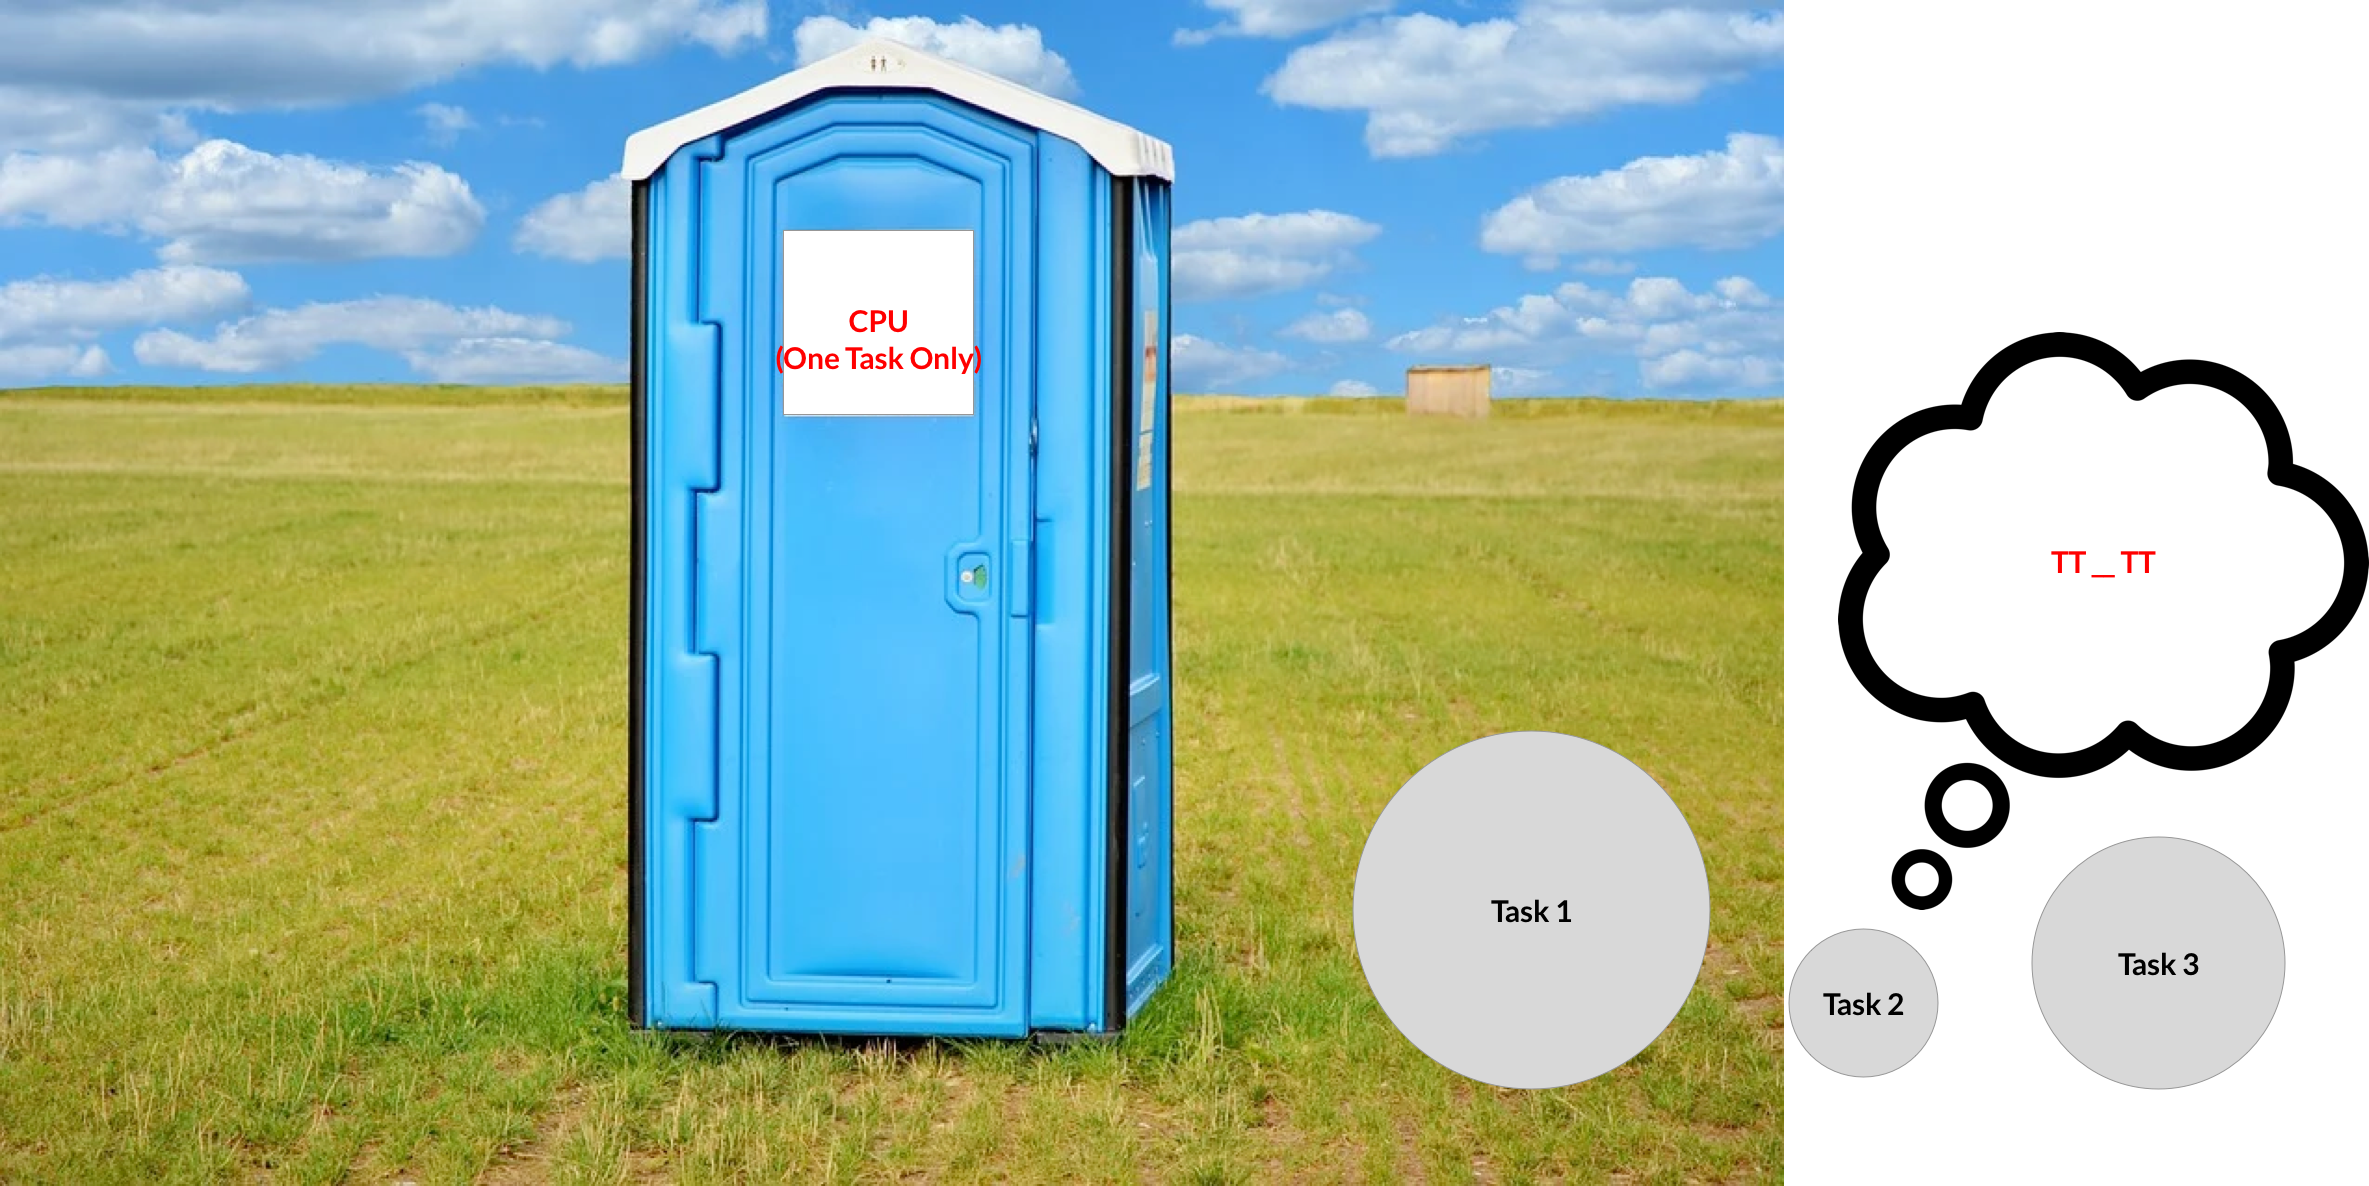
\includegraphics[width=0.8\linewidth]{../images/week_4_notes_1_1.png}
    \end{center}

    \underline{\textbf{References}}

    \begin{enumerate}[1)]
        \item Guru 99: What is CPU Scheduling?, \href{https://www.guru99.com/cpu-scheduling-algorithms.html#8}{link}
    \end{enumerate}

    \item Scheduling Algorithms: Shortest-Job-First
    \begin{itemize}
        \item Is also called \textbf{Shortest Remaining Time}
        \item Chooses the process with the shortest processing time
        \item Need to know processing time in advance
        \item Is applied in batch environments where short jobs are given preference $^{[1]}$
        \item Is NOT ideal method in a shared system where the required CPU time
        is not known $^{[1]}$
    \end{itemize}

    \bigskip

    \begin{center}
    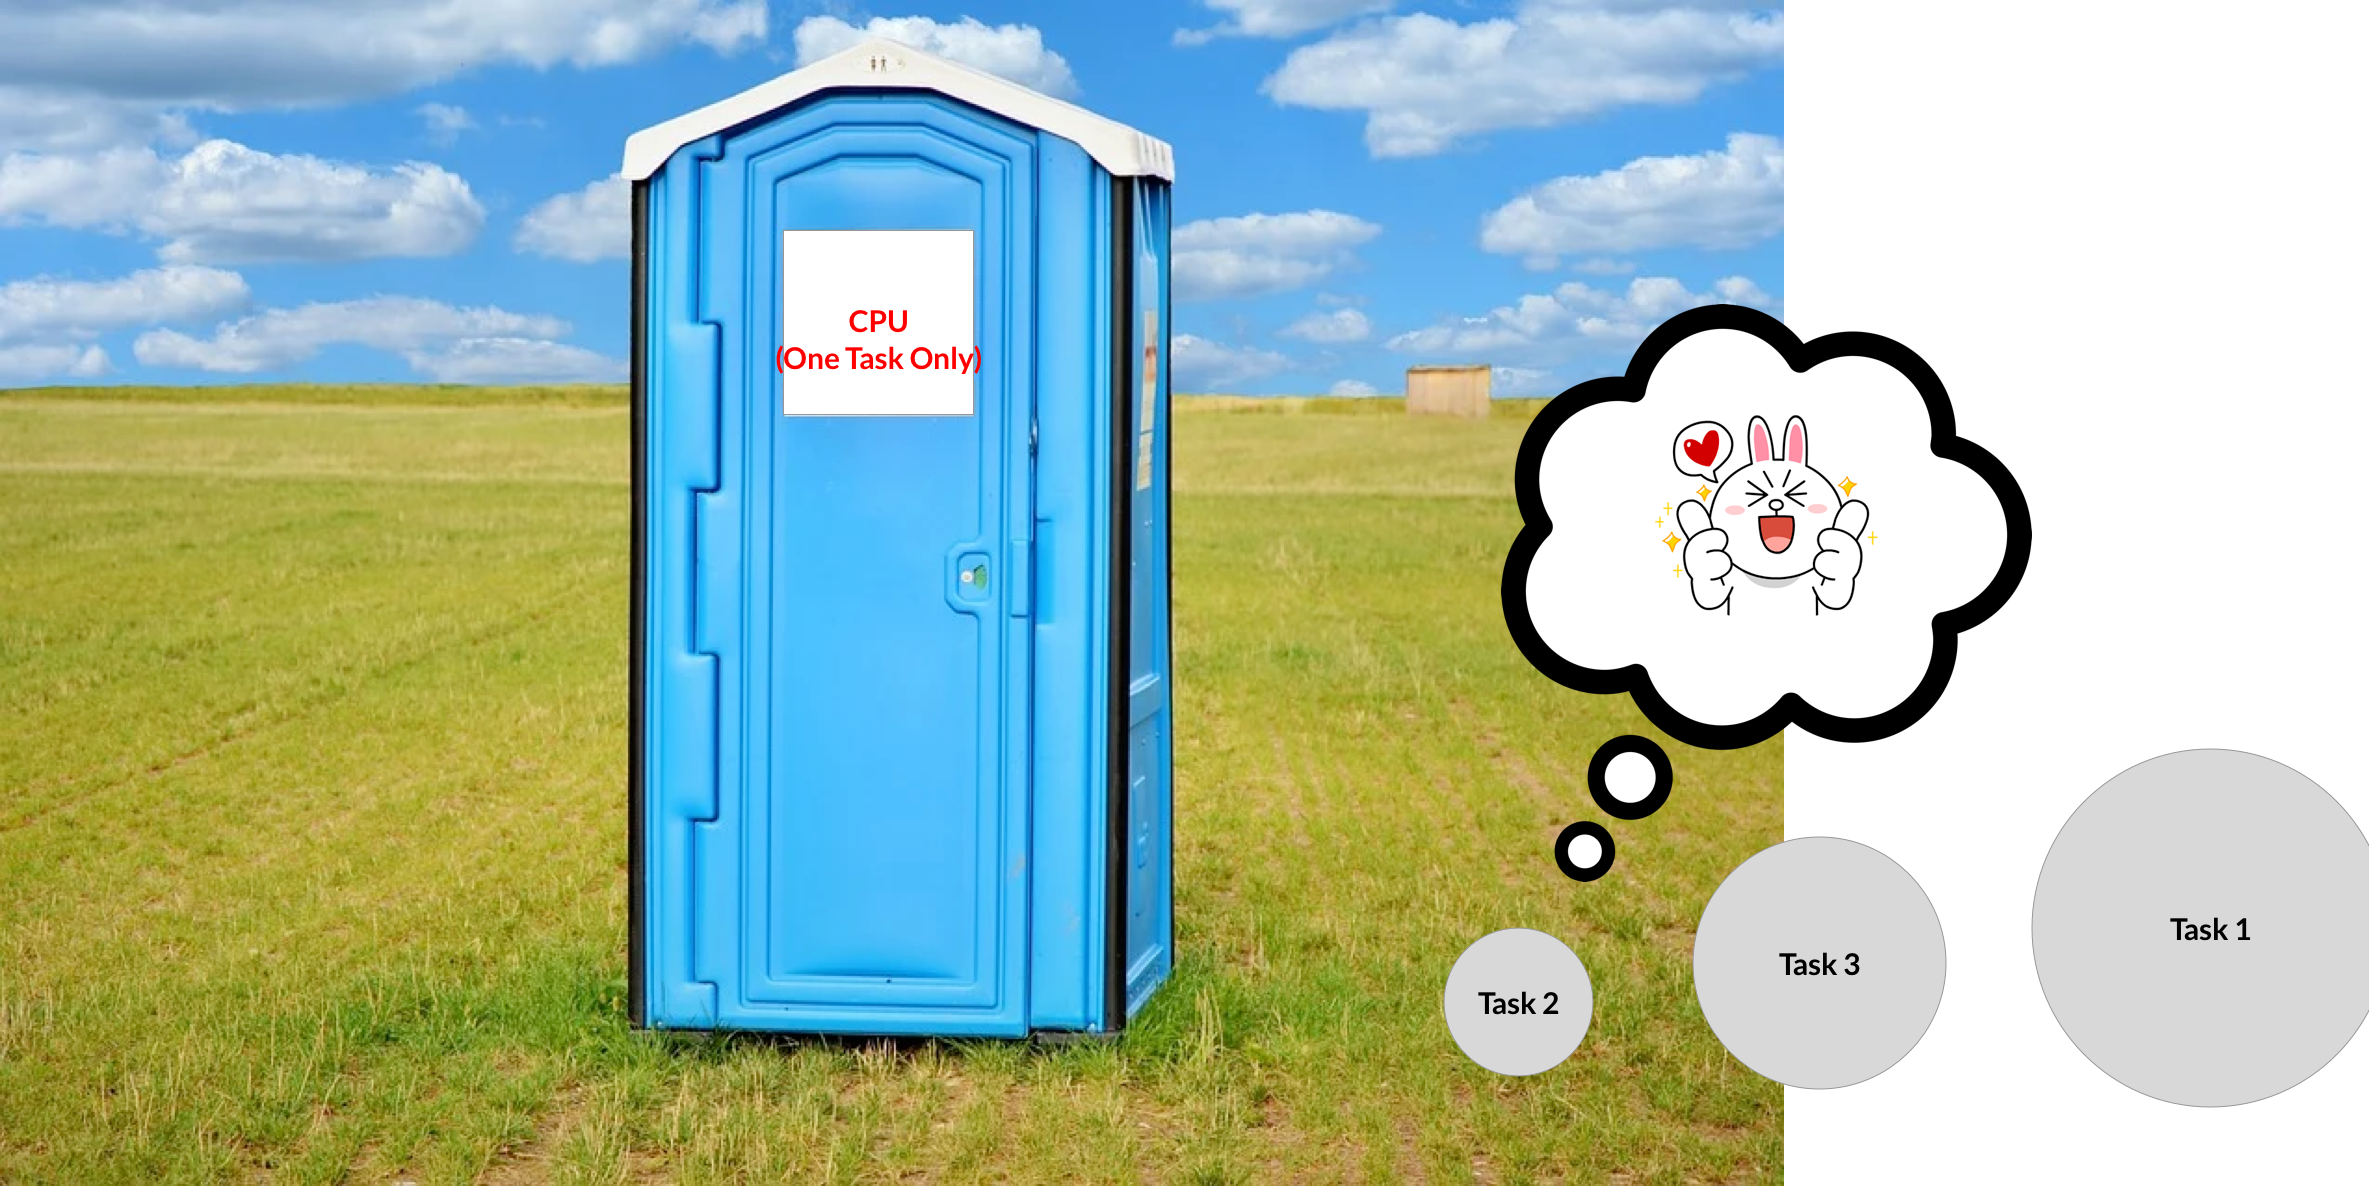
\includegraphics[width=0.8\linewidth]{../images/week_4_notes_1_2.png}
    \end{center}

    \underline{\textbf{References}}

    \begin{enumerate}[1)]
        \item Guru 99: What is CPU Scheduling?, \href{https://www.guru99.com/cpu-scheduling-algorithms.html#8}{link}
    \end{enumerate}

    \item Scheduling Algorithms: Round Robin
    \begin{itemize}
        \item Is oldest, simplest scheduling algorithm $^{[1]}$
        \begin{itemize}
            \item Each task gets equal share of CPU time
        \end{itemize}
        \item Is clock-driven $^{[1]}$
        \begin{itemize}
            \item e.g. After 100ms, current task is saved and pushed to last, and
            upcoming task is given prority
        \end{itemize}
        \item Is pre-emptive $^{[1]}$
        \item Is starvation-free $^{[2]}$
        \item Is mostly used for scheduling algorithms in multitasking. $^{[1]}$
    \end{itemize}

    \bigskip

    \begin{center}
    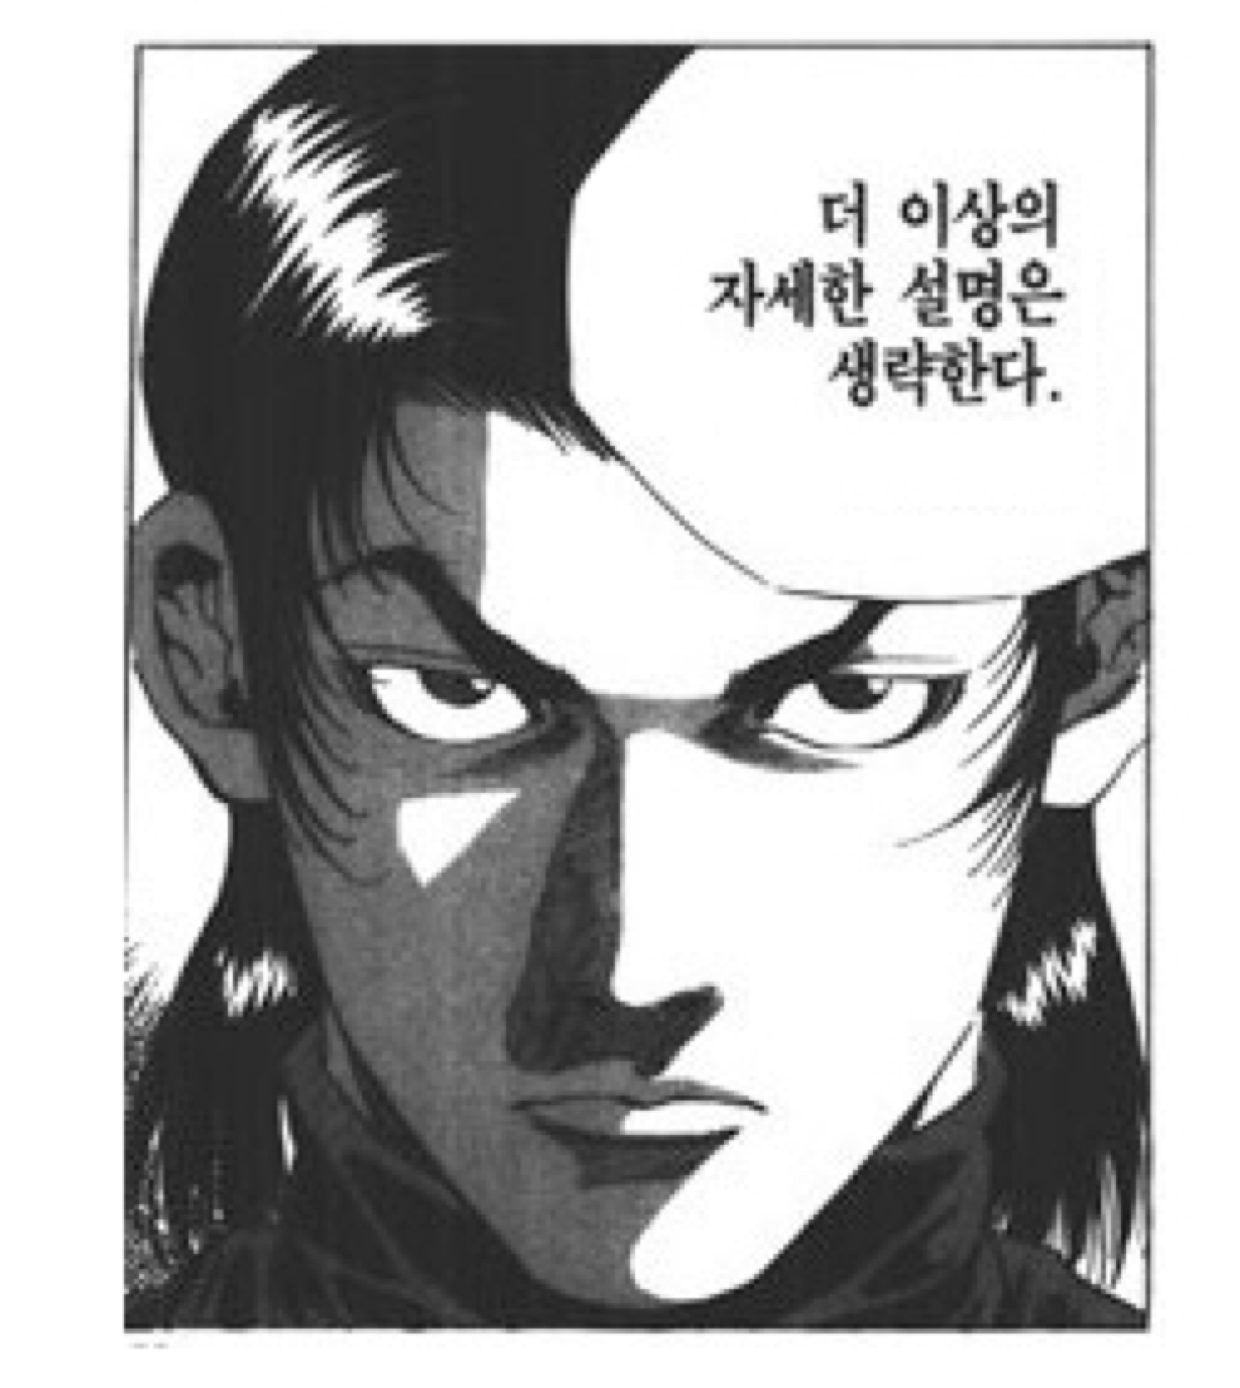
\includegraphics[width=0.5\linewidth]{../images/week_4_notes_1_3.png}
    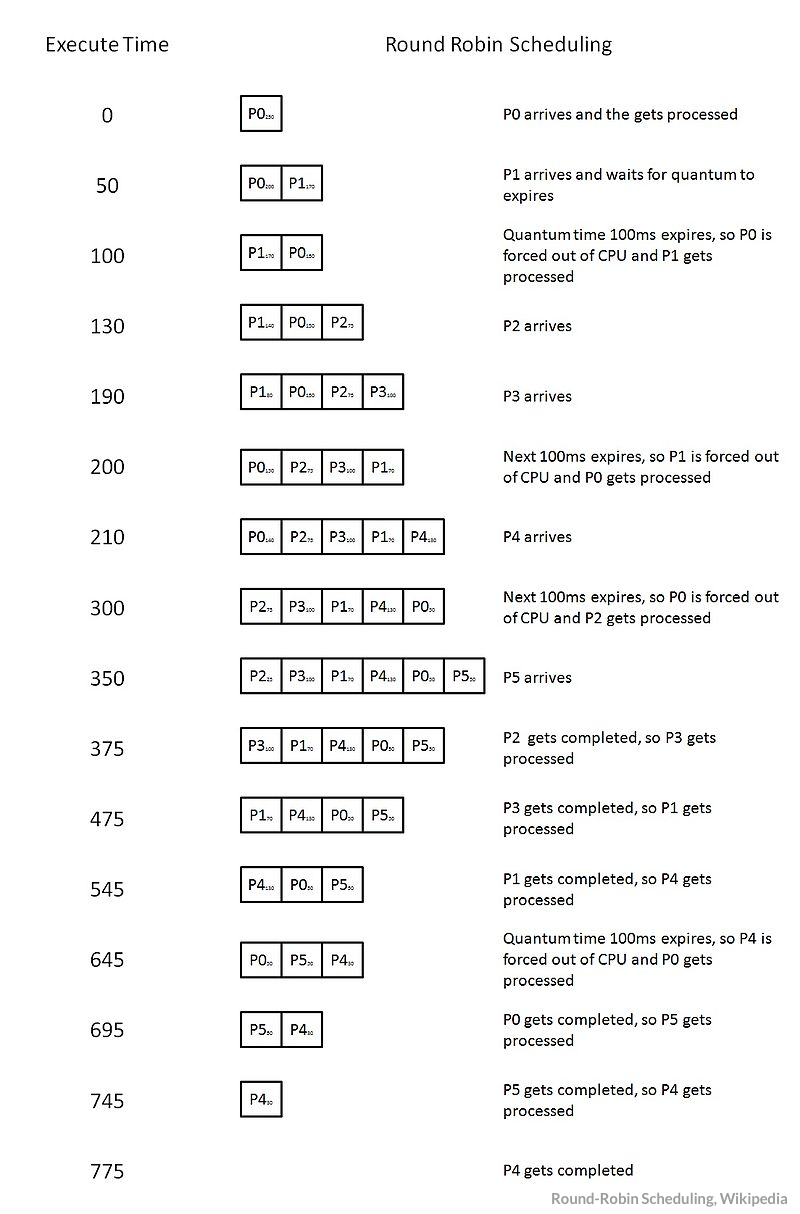
\includegraphics[width=0.8\linewidth]{../images/week_4_notes_1_4.png}
    \end{center}

    \underline{\textbf{References}}

    \begin{enumerate}[1)]
        \item Guru 99: What is CPU Scheduling?, \href{https://www.guru99.com/cpu-scheduling-algorithms.html#8}{link}
        \item Wikipedia: Round-robin Scheduling, \href{https://en.wikipedia.org/wiki/Round-robin_scheduling}{link}
    \end{enumerate}
    \item Scheduling Algorithms: Priority Scheduling

    \begin{itemize}
        \item Is a method of scheduling process based on priority $^{[1]}$
        \begin{itemize}
            \item Priority $p$ is associated with each process
            \item Highest priority job is selected from Ready state
            \item Priority can be based on memory requirements, time requirements, etc $^{[1]}$
        \end{itemize}
        \item Can be tricky
        \begin{itemize}
            \item Low priority task may never run
            \item Low priority task may prevent high priority task from making progress
            by holding resource (priority inversion)
        \end{itemize}
    \end{itemize}

    \underline{\textbf{References}}

    \begin{enumerate}[1)]
        \item Guru 99: What is CPU Scheduling?, \href{https://www.guru99.com/cpu-scheduling-algorithms.html#8}{link}
    \end{enumerate}

    % \item Priority Inversion
    \item Scheduling Algorithms: Multi-Level Queue Scheduling
    \begin{itemize}
        \item Permanently assigns processes to a queue $^{[2]}$
        \item Each queue have its separate scheduling algorithms $^{[1]}$
        \item Sets priorities for each queue $^{[1]}$
    \end{itemize}

    \begin{center}
    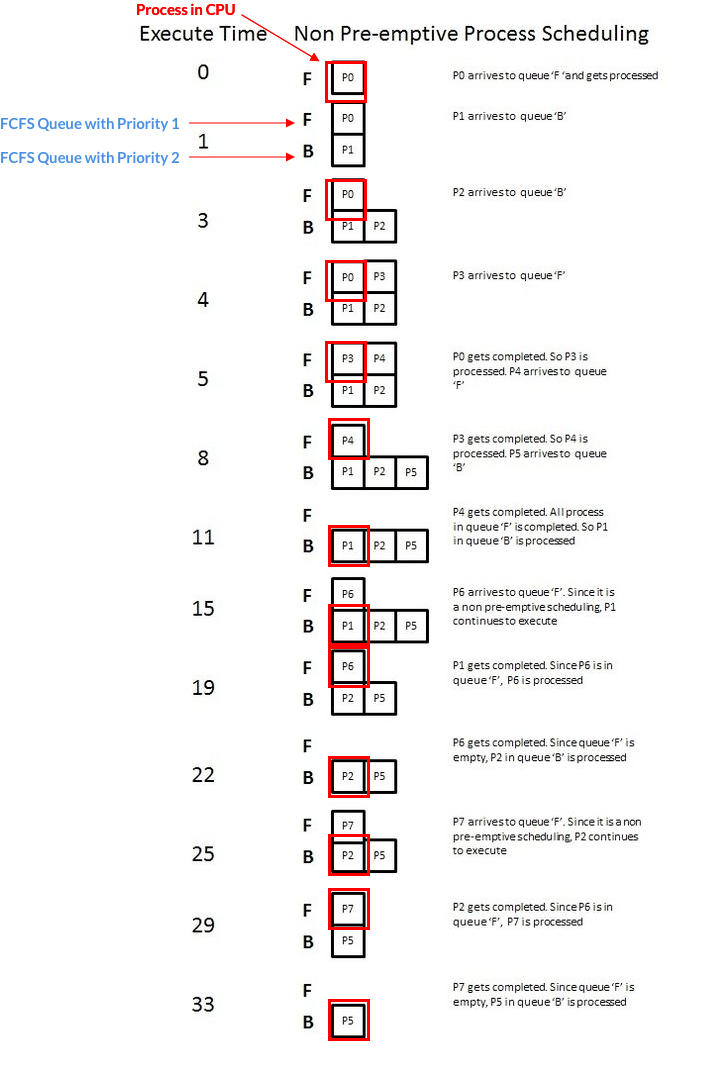
\includegraphics[width=0.8\linewidth]{../images/week_4_notes_1_5.png}
    \end{center}

    \bigskip

    \underline{\textbf{References}}

    \begin{enumerate}[1)]
        \item Guru 99: What is CPU Scheduling?, \href{https://www.guru99.com/cpu-scheduling-algorithms.html#8}{link}
        \item Wikipedia: Multilevel feedback queue, \href{https://en.wikipedia.org/wiki/Multilevel_feedback_queue}{link}
    \end{enumerate}

    \item Feedback Scheduling
    \begin{itemize}
        \item Is also called \textbf{Multi-level Feedback Queue} $^{[1]}$
        \item Meets the following design requirements for multinode systems $^{[1]}$
        \begin{enumerate}[1.]
            \item Give preference to short jobs
            \item Give preference to I/O bound processes
            \item Separate processes into categories based on their need for the
            processor
        \end{enumerate}
        \item Allows a process to move between queues $^{[1]}$
        \begin{itemize}
            \item e.g. Process in high-priority queue using too much CPU time $\to$ Lower-priority queues
        \end{itemize}
        \item e.g. Current Mac OS and Microsoft :)!! $^{[1]}$
    \end{itemize}

    \bigskip

    \underline{\textbf{References}}

    \begin{enumerate}[1)]
        \item Wikipedia: Multilevel feedback queue, \href{https://en.wikipedia.org/wiki/Multilevel_feedback_queue}{link}
    \end{enumerate}

    % \item Linux 2.6 CPU Scheduling
\end{itemize}

\end{document}